% Predlozak za pisanje diplomskog rada na PMF-MO
% Opcenita uputstva za LaTeX se mogu npr. naci na 
% http://web.math.hr/nastava/rp3, http://web.math.hr/nastava/s4-prof/latex.pdf
% NE PREPORUCA se "Ne baš tako kratak uvod u TEX", buduci se radi o vrlo starom prirucniku
% koji nije pogodan za moderne verzije LaTEXa.
% Originalna verzija "The not so short..." na http://tobi.oetiker.ch/lshort/lshort.pdf 
% je obnovljena i daje bolji uvid u moderne verzije LaTeXa

% Stil je optimiziran za kreiranje pdf dokumenta (npr. pomocu pdflatex-a, XeLaTeX-a)

\documentclass[a4paper,twoside,12pt]{memoir} % jednostrano: promijeniti twoside u oneside

% Paket inputenc omogucava direktno unosenje hrvatskih dijakritickih znakova 
% opcija utf8 za unicode (unix, linux, mac)
% opcija cp1250 za windowse
\usepackage[utf8]{inputenc}  % ukoliko se koristi XeLaTeX onda je \usepackage{xunicode}\usepackage{xltxtra}

% Stil za diplomski, unutra je ukljucena podrska za hrvatski jezik
\usepackage{diplomski}
% bibliografija na hrvatskom
\usepackage[languagenames,fixlanguage,croatian]{babelbib} % zahtijeva datoteku croatian.bdf
% hiperlinkovi 
\usepackage[pdftex]{hyperref} % ukoliko se koristi XeLaTeX onda je \usepackage[xetex]{hyperref}

% Odabir familije fontova:
% koristenjem XeLaTeX-a mogu se koristiti svi fontovi instalirani na racunalu, npr
% \defaultfontfeatures{Mapping=tex-text}
% \setmainfont[Ligatures={Common}]{Hoefler Text}
% ili
% \newcommand{\nas}[1]{\fontspec{Adobe Garamond Pro}\fontsize{24pt}{24pt}\color{Chocolate}\selectfont #1}
% i onda \nas{Naslov ...}
\usepackage{txfonts} % times new roman 

% Paket graphicx sluzi za manipuliranje grafikom 
\usepackage[pdftex]{graphicx} % ukoliko se koristi XeLaTeX onda je \usepackage[xetex]{graphicx}
% Paket amsmath je vec ukljucen
% Dodatno definirane matematicke okoline:
% teorem (okolina: thm), lema (okolina: lem), korolar (okolina: cor),
% propozicija (okolina: prop), definicija (okolina: defn), napomena (okolina: rem),
% slutnja (okolina: conj), primjer (okolina: exa), dokaz (okolina: proof)
% Definirane su naredbe za ispisivanje skupova N, Z, Q, R i C
% Definirane su naredbe za funkcije koje se u hrvatskoj notaciji oznacavaju drukcije 
% nego u americkoj: tg, ctg, ... (\tgh za tangens hiperbolni)
% Takodjer su definirane naredbe za Ker i Im (da bi se razlikovala od naredbe za imaginarni dio kompleksnog
% broja, naredba se zove \slika).

\pagestyle{headings}
% uz paket fancyhdr mogu se lako kreirati fancy zaglavlja i podnozja

% Podaci koje treba unijeti
\title{Paralelni algoritmi za problem grupiranja podataka}
\author{Anto Čabraja}
\advisor{prof. dr. sc. Goranka Nogo}  % obavezno s titulom (prof. dr. sc ili doc. dr. sc.)
\date{srpanj 2014.}  % oblika mjesec, godina

% Moguce je unijeti i posvetu
% Ukoliko nema posvete, dovoljno je iskomentirati/izbrisati sljedeci redak 
%\dedication{Samom sebi}

\begin{document}

% Naredna frontmatter generira naslovnu stranicu, stranicu za potpise povjerenstva, eventualnu posvetu i sadrzaj
% Moze se iskomentirati ukoliko nije u pitanju konacna verzija
\frontmatter

% Tekst diplomskog ...

% Diplomski rad treba poceti s uvodnim poglavljem  
\chapter*{Uvod}
\section[Problem grupiranja podataka][PGP]{Problem grupiranja podataka}
\section[Primjena][primjena]{Primjena}
\section[Pregled rada][pregled]{Pregled rada}

\chapter[Modeliranje problema grupiranja][MODELIRANJE]{Modeliranje problema grupiranja}	
% ukoliko naslov nije jako dugacak dovoljno je samo \chapter{Naslov poglavlja} 

\section[Osnovni pojmovi][os-pojmovi]{Osnovni pojmovi}
\label{sec:os-pojmovi}
Kako bi u daljnjem razmatranju bilo jednostavnije objašnjavati strukture i same implementacije algoritama potrebno je problem grupiranja reprezentirati osnovnim pojmovima. U nastavku ćemo formalno definirati sve komponente od kojih se problem grupiranja sastoji.
\begin{defn}
\label{def:uzorak}
\textbf{Uzorak} je apstraktna struktura podataka koja reprezentira stvarne podatke s kojima raspolaže algoritam za grupiranje.
\end{defn}
\begin{defn}
\label{def:svojstvo}
\textbf{Svojstvo} je vrijednost ili struktura koja predstavlja jednu značajku danog podatka unutar uzorka.
\end{defn}
\begin{defn}
\label{def:udaljenost}
\textbf{Udaljenost} između uzoraka definiramo kao funkciju 
$f: D  -> \R$, gdje je $D$ skup svojstava danih uzoraka
\end{defn}
\begin{defn}
\label{def:blizina}
Za uzorke kažemo da su \textbf{blizu} jedan drugome ako je njihova udaljenost manja od unaprijed zadane veličine
\end{defn}
\begin{defn}
\label{def:klaster}
\textbf{Klaster} je skup uzoraka koji su u prostoru podataka blizu. Ako su uzorci identični onda je njihova udaljenost uvijek $0$
\end{defn}
\begin{defn}
\label{def:hard}
\textbf{Jednistveno grupiranje} je postupak grupiranja kada svaki uzorak pripada jednom i samo jednom klasteru.
\end{defn}
\begin{defn}
\label{def:fuzzy}
\textbf{Nejasno ili nejedinstveno grupiranje} je postupak grupiranja gdje jedan uzorak može biti u više klastera.
\end{defn}
\begin{rem}
U radu ćemo promatrati \textbf{jedinstveno grupiranje} tako da će sve daljnje definicje i modeliranja predpostavljati da želimo dobiti disjunktne klastere. Jedinstveno grupiranje (eng: hard clustering) je ujedno i teži problem.
\end{rem}

\section[Matematičko modeliranje problema][MMP]{Matematičko modeliranje problema}
Definicija grupiranja podataka nije jedinstvena. U literati se na različite načine pokušava opisati ovaj postupak. Neki od pokušaja opisne definicije su:

\begin{enumerate}
\item \textit{Grupiranje podataka je postupak otkrivanja homogenih\footnote{podaci koji se ne mogu smisleno separirati} grupa uzoraka unutar skupa svih danih uzoraka.}

\item \textit{Grupiranje podataka je postupak određivanja koji su uzorci slični te ih svrstati u isti klaster.}
\end{enumerate}
Za modelirali problem neće nam biti dovoljne opisne definicije. U ovom slučaju opisne definicje mogu poslužiti samo kao intuicija o ćemu se zapravo radi kada govorimo o grupiranju. U nastavku ćemo pomoću definiranih pojmova u poglavlju \ref{sec:os-pojmovi} matematički opisati problem grupiranja podataka.

Neka je $\mathbf{U} = \{U_1,U_2,\cdots,U_n\} $ skup od $n$ uzoraka,te neka je $U_i = (s_1,s_2,\cdots,s_d)$ reprezentiran $d$-dimenzionalnim vektorom gdje $s_i$ predstavlja jedno svojstvo. Ovako definiran $\mathbf{U}$ moguće je reprezentirati kao matricu $\mathbf{S}_{d\times n}$.Svaki stupac te matrice predstavlja jedan uzorak iz danog skupa $\mathbf{U}$.
\begin{equation}
\label{equ:matrica-uzoraka}
\mathbf{S}_{d \times n} = 
\begin{pmatrix}
s_{1,1} & s_{1,2} & \cdots & \cdots & s_{1,n}\\
s_{2,1} & s_{2,2} & \cdots & \cdots & s_{2,n}\\
\vdots & \vdots & \ddots & \ddots & \vdots\\
s_{d,1} & s_{d,2} & \cdots & \cdots & s_{d,n}
\end{pmatrix}
\end{equation}
Iz definicje \ref{def:hard} te iz navedenog formalnog zapisa dajemo formalnu definiciju problema grupiranja.
\begin{defn}
\label{def:k-klaster}
\textbf{Skup od k klastera} $\mathbf{C} = \{C_1,C_2,...,C_k\}$ je skup sa sljedećim svojstvima:
\begin{itemize}
\item $C_i \neq \Phi$
\item $C_i \cap C_j = \Phi$ , $\forall i,j$ $ i \neq j$
\item $\cup_{i=1}^{k}C_i = \mathbf{U} $
\end{itemize} 
\end{defn}
\begin{rem}
\label{nap:ZC}
U terminima matrice $\mathbf{Z}$ to znači da se svaki $C_i$ zapravo sastoji od stupaca matrice $\mathbf{Z}$.
\end{rem}
\begin{defn}
\label{def:hard-formal}
\textbf{Problem grupiranja} u skup od k klastera $\mathbf{C}$ je ekvivalentan problemu da\\
$\forall c, c' \in C_i$ udaljenost od $c$ do $c'$ je manja od udaljenosti $c$ do bilo kojeg drugog $c'' \in C_j$ $ j \neq i$ 
\end{defn}
Zapravo problem grupiranja je pronalazak najpogodnije particije za $\mathbf{C}$ u skupu svih mogućih particija.
Prema napomeni \ref{nap:ZC} to znači da se zapravo radi o problemu raspodjele n stupaca matrice $\mathbf{Z}$ u $k$ skupova 
\section[Metode razvoja algoritama za grupiranje][metode razvoja]{Metode razvoja algoritama za grupiranje}
\section[Upravljanje podacima][upravljanje-podacima]{Upravljanje podacima}

\chapter[Metaheuristike]{Meta-heuristički pristup problemu}
\section[Prirodom inspirirani algoritmi][prirodni-algoritmi]{Prirodom inspirirani algoritmi}
\section{Reprezentacija podataka}
\section{Analiza rezultata}
\chapter{Poznati algoritmi i analiza}
\section{Alg 1}
\section{Alg 2}
\section{Alg 3}
\chapter{Tehnike za paralelizaciju algoritama}
\section[Osnovni pojmovi MPI tehnologije][mpi]{Osnovni pojmovi MPI tehnologije}
\section[Topologija][topologija]{Topologije}
\section[Prednosti paralelizacije i cijena komunikacije][pred-man-paralel]{Prednosti paralelizacije i cijena komunikacije}
\chapter{Konstrukcija paralelnih algoritama za grupiranje}
\section{Algoritam 1 heurisika}
\subsection{Opis}
\subsection{Analiza}
\section{Algoritam 2 iterativno}
\subsection{Opis}
\subsection{Analiza}
\section{Algoritam 3 hibrid}
\subsection{Opis}
\subsection{Analiza}
\chapter{Ostale moderne metode}
\section{Programiranje na grafičkim karticama}
\section{MapReduce metoda}
% Na kraju diplomkog rada stavlja se  bibliografija
% Najprije definiramo nacin prikazivanja bibliografije, u ovom slucaju verzija amsplain stila
\bibliographystyle{babamspl} % babamspl ili babplain

% U datoteku diplomski.bib se stavljaju bibliografske reference
% Bibliografske reference u bib formatu se mogu dobiti iz MathSciNet baze, Google Scholara, ArXiva, ...
\bibliography{diplomski}

\pagestyle{empty} % ne zelimo brojanje sljedecih stranica

% I na koncu idu sazeci na hrvatskom i engleskom

\begin{sazetak}
Ukratko ...
\end{sazetak}

\begin{summary}
In this ...
\end{summary}

% te zivotopis

\begin{cv}
Na slici \ref{def:fuzzy} se nalazi 3D graf neke funkcije. 

\begin{figure}[h!t]
\centering 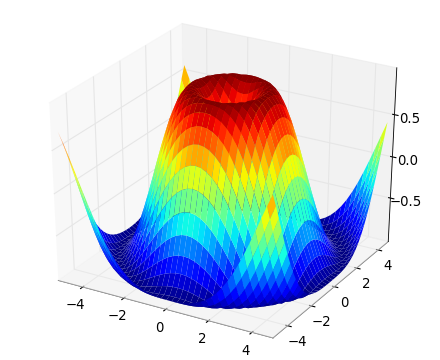
\includegraphics{surface3d.png}
\caption{Druga slika}
\label{fig:3d}
\end{figure}

kao i jedna vrlo komplicirana formula koja slijedi iz \eqref{eq:jed1}
\[ \sum_{i=1}^{\infty}A_{x_1}\times A_{{\alpha}_2}\oslash\iint_{\Omega}x^2\ddagger\limsup_{n\in\N}\frac{\alpha+\theta+\gamma}{n^{\omega}}\;\;\text{je u stvari}\;\;\biguplus_{r\in\Q}\overline{\Xi_i \mathop\Theta_{\substack{j\in\C \\ j\ni i\Q}} \Upsilon^{k^j} \underset{\ast}{\Psi} \hslash\vert_{\{\alpha\}}}.\]
\end{cv}

\end{document}